
\section{Methodology}The experiment was conducted using a standard impedance tube setup, closely following the methodology outlined in Utsuno's paper. This experiment differs primarily in its application: it is designed to measure the acoustic properties of 3D-printed porous media rather than natural materials such as sand. To start off a given experiment, a porous medium with known properties of pore length, pore shape, and pore size are placed in the impedance tube.

\subsection{Experimental Configuration}

The function generator seen in Fig. \ref{fig:Exp-setup} provides a signal to the speaker at one end of the impedance tube. A Python script controls the function generator, sweeping through frequencies from 150 Hz to 1,000 Hz in 10 Hz increments. At each frequency, the resulting sound wave is measured by two microphones. These microphones are connected to two differential preamplifiers to boost the signals before they are visualized and recorded on an oscilloscope. The oscilloscope captures the time-domain pressure signals, $p_1(t)$ and $p_2(t)$, which are then converted to the frequency domain to determine the complex pressures, $P_1$ and $P_2$, at each frequency. These complex pressures are required for Equation \ref{eq: microphone corrected transfer function}. To reduce measurement error, 16 oscilloscope averages are performed for each individual frequency. Additionally, for the oscilloscope to accurately distinguish between the 10 Hz frequency increments, the frequency resolution ($df$) must be smaller than 10 Hz. The frequency resolution is calculated using the following equation:
\begin{equation}
df = \frac{\text{sample rate}}{\text{number of samples}}
\end{equation}

The sampling rate on the oscilloscope is set to 50,000 samples/s, and the sample size is set to 10,000 samples. This yields a frequency resolution of 5 Hz, ensuring that when the time-domain signal is converted to the frequency domain, the resolution is enough to correctly identify between 10 Hz increments.

\begin{figure}[h!]
\centering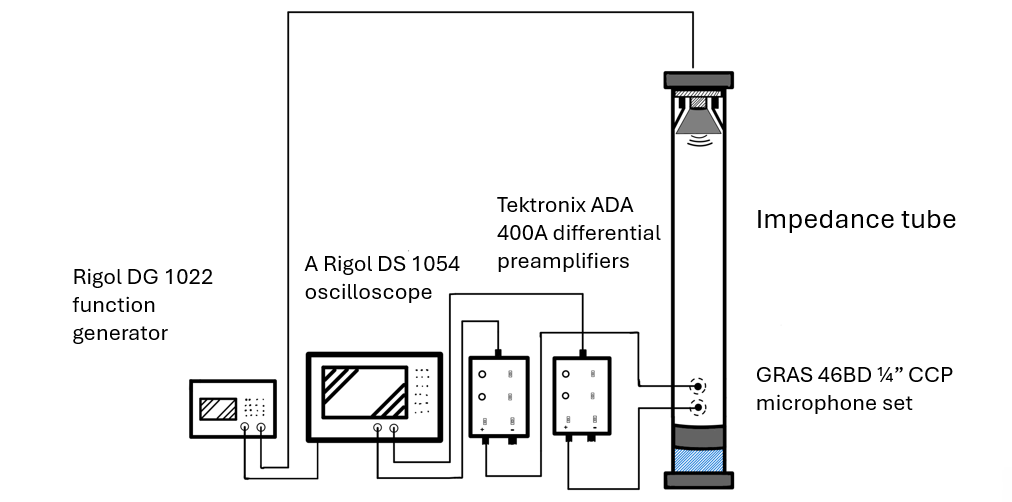
\includegraphics[width=0.8\linewidth]{Screenshot 2026-04-15 160511.png}
\caption{Experimental Setup}
\label{fig:Exp-setup}
\end{figure}

An important component of this setup, highlighted by the blue region at the bottom of the impedance tube in Fig. \ref{fig:Exp-setup}, is the interchangeable air backing ring. This is the ring used in the two cavity procedure.

\subsection{Two-Cavity Procedure}
A critical step in this method is varying the air backing depth. After the first frequency sweep is completed for an initial depth $D$, the air space ring at the back of the tube is replaced with a ring of a different depth, $D'$. As shown in Fig. \ref{fig:two_acoustic_environ}, this creates two unique acoustic environments within the tube.

\begin{figure}[h!]
\centering
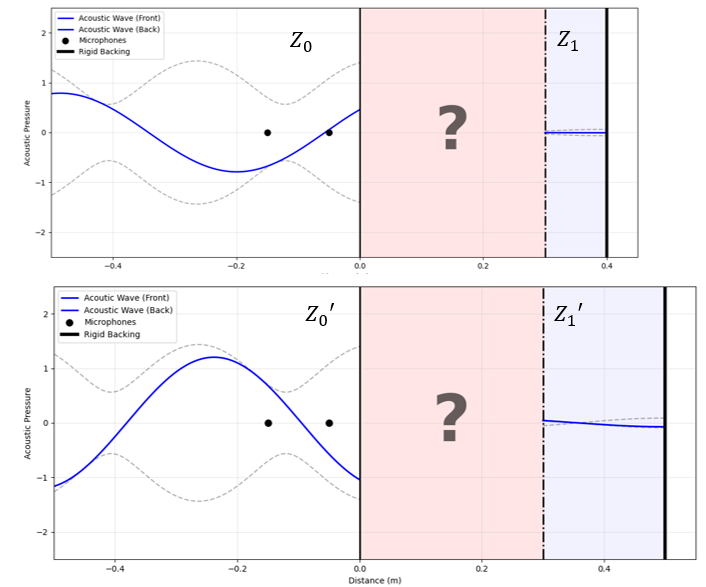
\includegraphics[width=0.7\linewidth]{Screenshot 2026-04-24 141326.png}
\caption{Two Unique Acoustic Environments}
\label{fig:two_acoustic_environ}
\end{figure}

This change in boundary conditions provides the modified impedance values, $Z_s'$ and $Z_b'$, which are necessary to calculate the characteristic impedance and propagation constant described by Equations \ref{char_impedance} and \ref{prop_constant}.

\subsection{Microphone correction}
\label{sec:Mic_correction}To account for and remove the inherent frequency response biases of the microphones, two frequency sweeps are performed for each air backing configuration. The first sweep is performed with the microphones in their standard configuration, giving a transfer function of:
\begin{equation}
H_{12} = \frac{\epsilon_1 P_{top}}{\epsilon_2 P_{bottom}}
\end{equation}

where $\epsilon_1$ and $\epsilon_2$ are the frequency responses associated with microphone 1 and microphone 2, respectively.The second measurement is performed with the microphone positions swapped. This results in a second transfer function:

\begin{equation}
H_{21} = \frac{\epsilon_2 P_{top}}{\epsilon_1 P_{bottom}}
\end{equation}

Combining these two frequency sweeps allows for the algebraic cancellation of the $\epsilon_1$ and $\epsilon_2$ terms, yielding the corrected transfer function, $H_{MC}$:

\begin{equation}
H_{MC} = \sqrt{H_{12} \cdot H_{21}} = \frac{P_{top}}{P_{bottom}}
\end{equation}
